\documentclass{article}
\usepackage[margin=0pt,paperwidth=32cm,paperheight=18cm]{geometry}
\usepackage{tikz}
\pagestyle{empty}

% ---------- 颜色 ----------
\definecolor{paper}{RGB}{240, 236, 220}     % 宣纸
\definecolor{green1}{RGB}{158, 188, 142}    % 远山：淡青绿
\definecolor{green2}{RGB}{105, 148, 100}    % 中山：中绿
\definecolor{green3}{RGB}{62, 100, 72}      % 近山：深绿
\definecolor{green4}{RGB}{32, 62, 48}       % 树：墨绿
\definecolor{ink}{RGB}{20, 30, 26}          % 墨
\definecolor{cinnabar}{RGB}{175, 60, 45}    % 朱砂

\begin{document}
\noindent
\begin{tikzpicture}[remember picture, overlay]
  \path (current page.south west) coordinate (SW);
  \begin{scope}[shift={(SW)}, x=1cm, y=1cm]

    % ==================== 宣纸底 ====================
    \fill[paper] (0,0) rectangle (32,18);

    % 细密纸纹
    \begin{scope}
      \clip (0,0) rectangle (32,18);
      \foreach \x in {0,0.8,...,32}
        \foreach \y in {0,0.8,...,18}
          \fill[ink, opacity=0.022] (\x,\y) circle (0.02);
    \end{scope}

    % ==================== 远山（最淡绿） ====================
    \fill[green1, opacity=0.48]
      (0,4)
      .. controls (3,12) and (5,14)  .. (8,11)
      .. controls (11,8) and (13,14) .. (16,14)
      .. controls (19,14) and (21,8) .. (24,11)
      .. controls (27,14) and (29,12) .. (32,9)
      -- (32,4) -- (0,4) -- cycle;

    % ==================== 中山（中绿） ====================
    \fill[green2, opacity=0.72]
      (0,4)
      .. controls (3,10) and (5,11.5) .. (8,9)
      .. controls (11,7) and (13,11.5) .. (16,11.5)
      .. controls (19,11.5) and (21,7) .. (24,9)
      .. controls (27,11.5) and (29,10) .. (32,7.5)
      -- (32,4) -- (0,4) -- cycle;

    % ==================== 近山（深绿） ====================
    \fill[green3, opacity=0.92]
      (0,4)
      .. controls (3,8) and (5,9)     .. (8,7)
      .. controls (11,5.5) and (13,9) .. (16,9)
      .. controls (19,9) and (21,5.5) .. (24,7)
      .. controls (27,9) and (29,8)   .. (32,6)
      -- (32,4) -- (0,4) -- cycle;

    % ==================== 山脚云雾 ====================
    \fill[paper, opacity=0.75] (0,3.5) rectangle (32,4.5);
    \fill[paper, opacity=0.45] (0,4.8) rectangle (32,5.2);
    \fill[paper, opacity=0.22] (0,6.5) rectangle (32,6.9);

    % ==================== 水面倒影 ====================
    \foreach \y/\op in {0.35/0.16, 0.90/0.13, 1.45/0.10, 2.00/0.075, 2.55/0.055, 3.10/0.04}{
      \draw[green3, opacity=\op, line width=0.4pt]
        (2,\y) .. controls (8,\y+0.10) and (14,\y-0.10) .. (20,\y)
               .. controls (24,\y+0.07) and (28,\y-0.07) .. (30,\y);
    }

    % ==================== 松树 ====================
    \def\pine#1#2#3#4{
      \begin{scope}[shift={(#1,#2)}, scale=#3, opacity=#4]
        % 树干
        \draw[ink, line width=0.5pt]
          (0,0) .. controls (0.06,0.6) and (-0.06,1.2) .. (0,1.8);
        % 枝干与松针
        \foreach \y/\ex in {1.50/0.50, 1.15/0.60, 0.80/0.55, 0.45/0.45}{
          \draw[ink, line width=0.3pt] (0,\y) -- (\ex,\y-0.08);
          \draw[ink, line width=0.3pt] (0,\y) -- (-\ex,\y-0.08);
          \fill[green4, opacity=0.80] (\ex,\y-0.10) circle (0.055);
          \fill[green4, opacity=0.80] (-\ex,\y-0.10) circle (0.055);
        }
        \fill[green4, opacity=0.80] (0,1.82) circle (0.07);
      \end{scope}
    }

    \pine{1.2}{5.5}{1.05}{0.92}
    \pine{2.6}{6.4}{0.85}{0.88}
    \pine{4.0}{7.2}{0.68}{0.80}

    % ==================== 飞鸟 ====================
    \foreach \x/\y/\s in {20.0/15.1/0.20, 21.1/15.4/0.16, 22.1/15.0/0.14, 23.0/15.3/0.12}{
      \draw[ink, opacity=0.35, line width=0.55pt]
        (\x,\y) .. controls (\x+0.12,\y+\s) and (\x+0.22,\y+\s) .. (\x+0.32,\y)
                .. controls (\x+0.42,\y+\s) and (\x+0.52,\y+\s) .. (\x+0.64,\y);
    }

    % ==================== 朱砂印章 ====================
    \fill[cinnabar, opacity=0.85] (29.2,1.2) rectangle (30.8,2.8);
    \draw[paper, opacity=0.90, line width=0.6pt] (29.2,2.0) -- (30.8,2.0);
    \draw[paper, opacity=0.90, line width=0.6pt] (30.0,1.2) -- (30.0,2.8);
    \draw[paper, opacity=0.45, line width=0.3pt] (29.35,1.35) rectangle (30.65,2.65);

  \end{scope}
\end{tikzpicture}
\end{document}
